\documentclass[12pt, xcolor=dvipsnames,svgnames,x11names]{article}

\input{common}

\renewcommand{\familydefault}{\sfdefault}


% Redefine \maketitle to include tcolorbox
\makeatletter
\renewcommand{\maketitle}{%
      \begin{center}
         \begin{tcolorbox}[
               enhanced,
               colback=white,
               colframe=stormblue,
               boxrule=1pt,
               arc=3pt,
               left=0pt,
               right=0pt,
               top=0pt,
               bottom=0pt,
               drop shadow={goldenrod!25!white},
         ]
               % Header section
               \begin{tcolorbox}[
                  enhanced,
                  colback=goldenrod,
                  colframe=goldenrod,
                  boxrule=0pt,
                  arc=3pt,
                  sharp corners=south,
                  left=2em,
                  right=2em,
                  top=1em,
                  bottom=1em
               ]
                  \centering
                  {\LARGE\bfseries\textcolor{white}{\@title}}
               \end{tcolorbox}
               
               % Content section
               \vspace{1em}
               \centering
               {\large\textcolor{darkgray}{\@author}} \\[0.8em]
               {\normalsize\textcolor{darkgray}{\@date}}
               \vspace{1em}
         \end{tcolorbox}
      \end{center}
      \vspace{2em}
}
\makeatother



\newcommand{\hw}{Homework 2: Operations on Signals}
\newcommand{\duedate}{Sept 27, 2026, 11:59 PM}
\newcommand{\hwturnin}{hw01}

\newenvironment{multiequation}[1][]{%
\begin{equation}%
   \begin{aligned}%
   \ifx#1\@empty\else\label{#1}\fi%
}{%
   \end{aligned}%
\end{equation}%
}
\pagestyle{fancy}

\lhead{\footnotesize{\coursenumber, \courseterm}}
\chead{}
\rhead{\footnotesize{\emph{\hw}}}
\lfoot{\footnotesize{\instructorname}}
\cfoot{\footnotesize{\thepage}}
\rfoot{\footnotesize{\textit{Last Revised:~\today}}\\ \footnotesize{The University of Alabama in Huntsville}}
\renewcommand{\headrulewidth}{0.1pt}
\renewcommand{\footrulewidth}{0.1pt}
\newcommand{\minipagewidth}{0.8\columnwidth}

\renewcommand{\thefootnote}{\fnsymbol{footnote}}


\renewcommand{\headrulewidth}{0.1pt}
\renewcommand{\footrulewidth}{0.1pt}

\renewcommand{\thefootnote}{\fnsymbol{footnote}}

\newcommand{\showanswers}{no}

\begin{document}


\title{\textsc{\hw\\
\coursenumber}}
\author{Instructor: \instructorname}
\date{Due: \duedate\\ 116 points}

\maketitle

\setlength{\unitlength}{1in}
You are allowed to use a generative model-based AI tool for your assignment. However, you must submit an accompanying reflection report detailing how you used the AI tool, the specific query you made, and how it improved your understanding of the subject. You are also required to submit screenshots of your conversation with any large language model (LLM) or equivalent conversational AI, clearly showing the prompts and your login avatar. Some conversational AIs provide a way to share a conversation link, and such a link is desirable for authenticity. Failure to do so may result in actions taken in compliance with the plagiarism policy.

Additionally, you must include your thoughts on how you would approach the assignment if such a tool were not available. Failure to provide a reflection report for every assignment where an AI tool is used may result in a penalty, and subsequent actions will be taken in line with the plagiarism policy.

\subsection*{Submission instruction:}
Upload a .pdf on Canvas with the format  \texttt{CPE381-LastFirst-HW-XX}. For example, if your name is Sam Wells, your file name should be \texttt{CPE381-WellsSam-HW-XX.pdf}.  If there is a programming assignment, then you should include your source code along with your PDF files in a zip file \texttt{CPE381-LastFirst-HW-XX.zip}. 
Your submission must contain your name and UAH Charger ID or your UAH email address.  Please number your pages as well.
\vskip 1em
\hrule
\vskip 1em


{{\LARGE \textbf{Theory}}}


\section{Linear Interpolation (6 Points)}
Assume three signal values  $x = \{3.0, 4.0, 3.5\}$ at timestamp $t = \{ 2.0, 4.0, 6.0\}$.  We will consider the case of linear interpolation.

\begin{enumerate}
\item How many linear segments are required if given three samples or signal values? \textbf{(2 Points)}
\item Write down all the equation of line segments necessary for linear interpolation given the three samples above. \textbf{(2 Points)}
\item  What is the value of when interpolated at $t = 2.5$?  \textbf{(2 Points)}
\end{enumerate}

\section{Cubic Spline Interpolation (10 Points)}

Consider signal values $x = \{0.0, 7.0, 9.0, 3.0, 4.0\}$ at timestamp $t = \{ 0.0, 1.0, 2.0, 4.0, 5.0\}$.  We will consider the case of cubic spline interpolation.

\begin{enumerate}
\item Assuming free boundary condition, write the $B$ matrix corresponding to all the $b_i$ coefficients as per formulation provided in Chapter 02 Slides. \textbf{(6 Points)}

\item What are the values of $a_1$, $b_1$, $c_1$, $d_1$ following the convention for cubic spline interpolation formulation as described in the Chapter 02 slides? \textbf{(4 Points)}

\end{enumerate}


\section{Play with Signals. (10 points)} 
A continuous-time signal x( t) is shown in Figure~\ref{fig:hw02_Q1}.
\begin{figure}[htpb]
\centering
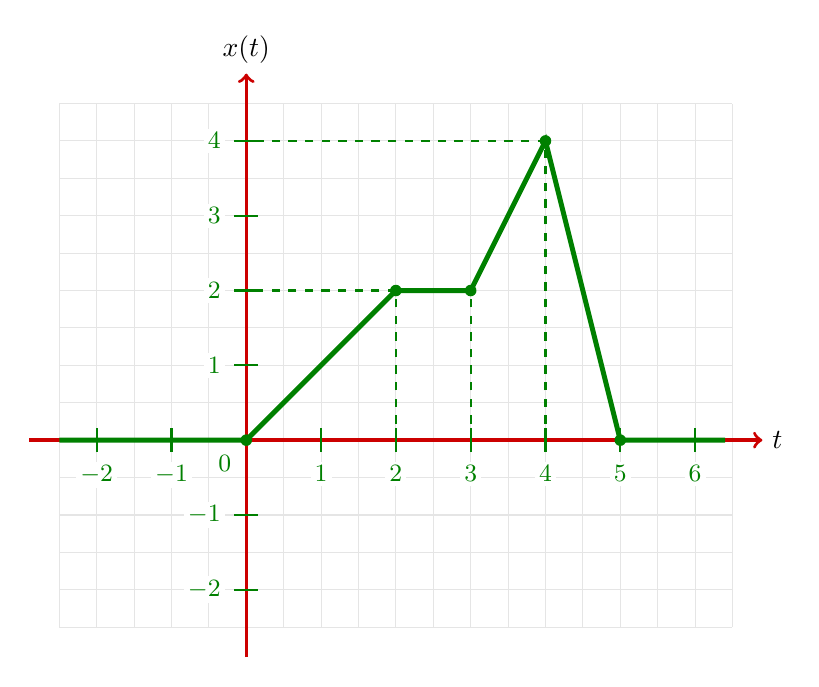
\begin{tikzpicture}[
    scale=0.95,
    axisline/.style={red!80!black, line width=1.2pt, ->},
    curve/.style={green!50!black, line width=1.8pt},
    guide/.style={green!50!black, thick, dashed},
    lbl/.style={green!50!black, font=\small\bfseries,
                fill=white, inner sep=1.5pt}
]

% ---------- grid ----------
\draw[lightgray!40, thin, step=0.5] (-2.5,-2.5) grid (6.5,4.5);

% ---------- axes ----------
\draw[axisline] (-2.9,0) -- (6.9,0) node[right, black, inner sep=3pt] {$t$};
\draw[axisline] (0,-2.9) -- (0,4.9) node[above, black, inner sep=3pt] {$x(t)$};

% ---------- guides to the breakpoints ----------
\draw[guide] (2,0) -- (2,2) -- (0,2);
\draw[guide] (3,0) -- (3,2);
\draw[guide] (4,0) -- (4,4) -- (0,4);

% ---------- signal ----------
\draw[curve] (-2.5,0) -- (0,0) -- (2,2) -- (3,2) -- (4,4) -- (5,0) -- (6.4,0);

% ---------- breakpoints ----------
\foreach \p in {(0,0),(2,2),(3,2),(4,4),(5,0)}
  \fill[green!50!black] \p circle (2.2pt);

% ---------- ticks, all four quadrants ----------
\foreach \u in {-2,-1,1,2,3,4,5,6}
  \draw[green!50!black, thick] (\u,-0.16) -- (\u,0.16);
\foreach \v in {-2,-1,1,2,3,4}
  \draw[green!50!black, thick] (-0.16,\v) -- (0.16,\v);

% ---------- tick labels ----------
\foreach \u in {-2,-1,1,2,3,4,5,6}
  \node[lbl, anchor=north] at (\u,-0.28) {$\u$};
\foreach \v in {-2,-1,1,2,3,4}
  \node[lbl, anchor=east] at (-0.28,\v) {$\v$};
\node[lbl, anchor=north east] at (-0.14,-0.14) {$0$};

\end{tikzpicture}
\caption{The ramp rises with unit slope
until $t=2$, holds the value $2$ over $2\le t\le 3$, climbs with slope $2$ to
its peak of $4$ at $t=4$, and falls to zero at $t=5$.}
\label{fig:hw02_Q1}
\end{figure}
\newline Based on $x(t)$ plot, sketch and label each of the following signals: (i) $x(t-2)$; (ii) $x(2t)$; (iii) $x(t/2)$; (iv) $x(-t)$; (v) $-x(-t)$.

\ifthenelse{\equal{\showanswers}{yes}}
{
\newpage
\subsection{Answers:}

\begin{figure}[htpb]
\centering
\includegraphics[width=0.99\linewidth, trim={0cm 0.0cm 0cm 0.0cm},clip]{figures/hw02_A1.pdf}
\caption{\textbf{Play with Signals} Answer}
\label{fig:hw02_A1}
\end{figure}

}

\section{Picasso of Signals (15 points)}
Sketch the following signals:
\begin{enumerate}
    \item $x(t) = u(t) - u(t - a)$, \quad $ a > 0$
    \item $y(t) = t [ u(t) - u(t - a) ]$, $a > 0$
    % \item $z(t) = \textrm{sgn}(t) = 1, \text{if}~ t > 0, \text{else}~ -1$

    % \begin{equation*}
    %     \begin{aligned}
    %         z(t) = \textrm{sgn}(t) = \begin{cases}
    %              1, \quad \text{}~ t > 0\\
    %              -1 \quad \text{otherwise}
    %         \end{cases}
    %     \end{aligned}
    % \end{equation*}
    \item $z(t) = u(-t) - u(t)$
    where $u(t)$ is the unit-step signal.
    
    % Note: sgn function is shortened notation for sign function which gives -1 if the argument is negative, and +1 if the argument is positive.
\end{enumerate}

\ifthenelse{\equal{\showanswers}{yes}}
{
\newpage
\subsection{Answers:}

\begin{figure}[htpb]
\centering
\includegraphics[width=0.4\linewidth, trim={1cm 9.0cm 14cm 1.0cm},clip]{figures/hw02_Q2.pdf}
\includegraphics[width=0.3\linewidth, trim={0cm 0.0cm 0.0cm 0.0cm},clip]{figures/CPE381_FA24_HW02_Q2_3.pdf}
\caption{Q2 Answer}
\label{fig:hw02_Q2}
\end{figure}

}

\section{Divide and Conquer (10 points)}
Determine the even and odd components of the following signals:
\begin{enumerate}
    \item $x(t) = u(t)$.
    \item $x(t) = \sin\bigg({\omega_0 t + \frac{\pi}{4}}\bigg) $
\end{enumerate}

\ifthenelse{\equal{\showanswers}{yes}}
{
\subsection{Answers:}
\begin{enumerate}
    \item $x_e(t) = \frac{1}{2}$,  $x_o(t) = \frac{1}{2} \textrm{sgn}(t)$
    \item $x_e(t) = \frac{1}{\sqrt{2}} \cos(\omega_0 t)$, 
  $x_o(t) = \frac{1}{\sqrt{2}} \sin(\omega_0 t)$
\end{enumerate}
}

\section{Rinse and Repeat (15 points)}
Determine whether or not each of the following signals is periodic. If signals are periodic, find their fundamental period.

\begin{enumerate}
    \item $x(t) = \cos\bigg( 2t + \frac{\pi}{4}\bigg)$.
    \item $x(t) = \cos^2(t)$.
    \item $x(t) = \cos(2\pi t) u(t)$.
\end{enumerate}

\ifthenelse{\equal{\showanswers}{yes}}
{
\subsection{Answers:}
\begin{enumerate}
    \item Periodic, period = $\pi$.
    \item Periodic, period = $\pi$.
    \item Nonperiodic.
\end{enumerate}
}



{{\LARGE \textbf{Practice}}}


\section{MATLAB Programming: Signal Plotting (10 points)}
% Q1.26 (a) and (b) only, Chapter 1 of the Textbook ``Signal and Systems using MATLAB" by Chaparro \& Akan.

Consider 

$$
y(t) = A\cos(\Omega_c t + s(t))
$$

\begin{enumerate}
    \item $ A = 1$, $\Omega_c = 2$, $s(t) = \tfrac{t^2}{4}$. Use MATLAB to plot the signal for $0 \leq t \leq 40$ seconds in the steps of $0.05$. Use \texttt{sound} function to listen to the signal.
 \item $ A = 1$, $\Omega_c = 2$, $s(t) = -2\sin(t)$. Use MATLAB to plot the signal for $0 \leq t \leq 40$ seconds in the steps of $0.05$. %Use \texttt{sound} function to listen to the signal.
\end{enumerate}

%\subsection{Answers:}
%\begin{minted}
%[
%frame=lines,
%framesep=2mm,
%baselinestretch=1.2,
%bgcolor=LightGray,
%fontsize=\footnotesize
%]
%{matlab}
%
%t=0:0.05:40;
%
%y=cos(2*t+t.^2/4);
%y1=cos(2*t- 2*sin(t));
%fig = figure(14)
%subplot(211)
%plot(t,y); title('Part 1: linear chirp')
%axis([0 20 1.1*min(y) 1.1*max(y)]);grid
%subplot(212)
%plot(t,y1);title('Part 2: sinusoidal chirp');xlabel('t')
%axis([0 20 1.1*min(y1) 1.1*max(y1)]);grid
%
%sound(y);
%sound(y1);
%
%\end{minted}
%
%
%\begin{figure}[htpb]
%\centering
%
%\includegraphics[width=0.6\linewidth, trim={0cm 0.0cm 0cm 0.0cm},clip]{figures/HW02_Q5.pdf}
%
%
%\caption{MATLAB Programming: Signal Plotting}
%\label{fig:HW02_Q5}
%\end{figure}


\section{Compact Form (20 points)}
For Figure~\ref{fig:HW02_Q6_CPE381_FA24}, represent the signal $(f)$ in compact form using transformed version of unit-step function $u(t)$ and ramp signal $r(t)$ as necessary.

\begin{figure}[htpb]
\centering
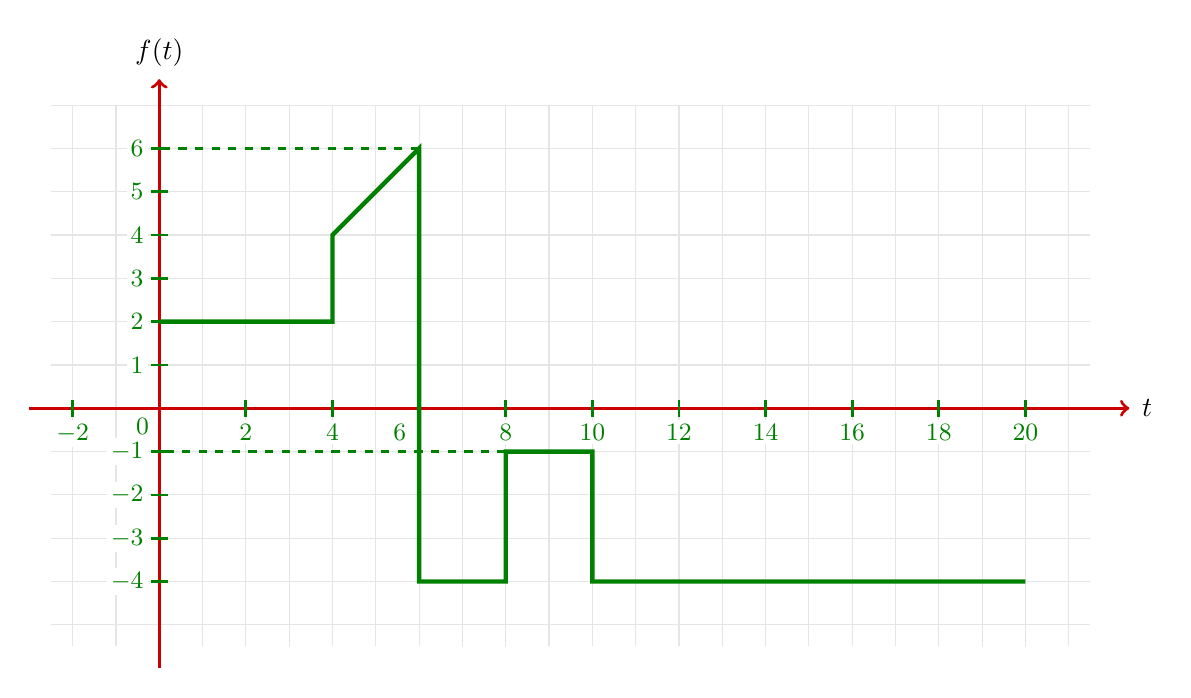
\begin{tikzpicture}[
    x=0.55cm, y=0.55cm,
    axisline/.style={red!80!black, line width=1.2pt, ->},
    curve/.style={green!50!black, line width=1.6pt},
    guide/.style={green!50!black, thick, dashed},
    lbl/.style={green!50!black, font=\small\bfseries,
                fill=white, inner sep=1.5pt},
    tick/.style={green!50!black, line width=1pt}
]

% ---------- grid ----------
\draw[lightgray!40, thin, step=1] (-2.5,-5.5) grid (21.5,7);

% ---------- axes ----------
\draw[axisline] (-3,0) -- (22.4,0) node[right, black, inner sep=4pt] {$t$};
\draw[axisline] (0,-6) -- (0,7.6) node[above, black, inner sep=4pt] {$f(t)$};

% ---------- guides ----------
\draw[guide] (6,6) -- (0,6);
\draw[guide] (8,-1) -- (0,-1);

% ---------- signal, right continuous at every jump ----------
\draw[curve]
      (0,2) -- (4,2) -- (4,4) -- (6,6) -- (6,-4) -- (8,-4)
   -- (8,-1) -- (10,-1) -- (10,-4) -- (20,-4);

% ---------- ticks in all quadrants ----------
\foreach \u in {-2,2,4,6,8,10,12,14,16,18,20}
  \draw[tick] ([yshift=-3pt]\u,0) -- ([yshift=3pt]\u,0);
\foreach \v in {-4,-3,-2,-1,1,2,3,4,5,6}
  \draw[tick] ([xshift=-3pt]0,\v) -- ([xshift=3pt]0,\v);

% ---------- tick labels ----------
\foreach \u in {-2,2,4,8,10,12,14,16,18,20}
  \node[lbl, below=4pt] at (\u,0) {$\u$};
% the jump at t=6 crosses the axis, so its label steps aside
\node[lbl, below=4pt, xshift=-7pt] at (6,0) {$6$};
\foreach \v in {-4,-3,-2,-1,1,2,3,4,5,6}
  \node[lbl, left=4pt] at (0,\v) {$\v$};
\node[lbl, anchor=north east, xshift=-2pt, yshift=-2pt] at (0,0) {$0$};

\end{tikzpicture}

\caption{Compact Form}
\label{fig:HW02_Q6_CPE381_FA24}
\end{figure}

Write a MATLAB script to produce Figure~\ref{fig:HW02_Q6_CPE381_FA24}. Note that the signal for $t < 0$ is zero.

\textbf{Tip:} You may use \texttt{heaviside} function in MATLAB to implement $u(t)$.

%\subsection{Answers:}
%
%\textbf{Option 1:}
%
%
%\begin{minted}
%[
%frame=lines,
%framesep=2mm,
%baselinestretch=1.2,
%bgcolor=LightGray,
%fontsize=\footnotesize
%]
%{matlab}
%
%
%% Define the time vector with a step of 0.01
%t = 0:0.01:20;
%
%% Initialize the function values
%f = zeros(size(t));
%
%% Define the piecewise function
%for i = 1:length(t)
%    if t(i) > 0 && t(i) <= 4
%        f(i) = 2;
%    elseif t(i) > 4 && t(i) <= 6
%        f(i) = t(i);
%    elseif t(i) > 6
%        f(i) = -4;
%    end
%end
%
%% Create the plot
%fig = figure;
%fig.Position= [421         632        1139         606];
%plot(t, f, 'LineWidth', 2);
%xlabel('t', 'FontSize', 24, 'Interpreter', 'latex');
%ylabel('f(t)', 'FontSize', 24, 'Interpreter', 'latex');
%title('HW02 Q6 CPE381 FA24', 'FontSize', 24, 'Interpreter', 'latex');
%grid on;
%axis equal
%set(gca, 'FontSize', 16);
%
%\end{minted}
%
%
%\textbf{Option 2:}
%
%
%\begin{minted}
%[
%frame=lines,
%framesep=2mm,
%baselinestretch=1.2,
%bgcolor=LightGray,
%fontsize=\footnotesize
%]
%{matlab}
%
%%% Alternatively
%
%% Define the time vector with a step of 0.01
%t = 0:0.01:20;
%
%% Define the piecewise function using unit-step (Heaviside) and ramp functions (t)
%f = 2 * (heaviside(t) - heaviside(t - 4)) + (t) .* (heaviside(t - 4) - 
%	heaviside(t - 6)) - 4 * heaviside(t - 6);
%
%% Create the plot
%fig = figure;
%fig.Position= [421         632        1139         606];
%plot(t, f, 'LineWidth', 2);
%xlabel('t', 'FontSize', 24, 'Interpreter', 'latex');
%ylabel('f(t)', 'FontSize', 24, 'Interpreter', 'latex');
%title('HW02 Q6 CPE381 FA24', 'FontSize', 24, 'Interpreter', 'latex');
%grid on;
%axis equal;
%set(gca, 'FontSize', 16);
%
%\end{minted}

%\section{Differential Equation in Practice}
%
%Consider an RL Circuit as shown in Figure~\ref{fig:RL_Circuit}.
%
%\begin{figure}[htpb]
%\centering
%\includegraphics[width=0.4\linewidth, trim={0cm 0.0cm 0cm 0.0cm},clip]{figures/RL_Circuit.pdf}
%\caption{Q1}
%\label{fig:RL_Circuit}
%\end{figure}


\section{Cubic Spline Interpolation and Data-fitting (20 Points)}

Consider renewable energy based electric grid and weather data for 1 week starting from 1/1/2018 12:00:00 AM in the zone 1 of ERCOT (Electric Reliability Council of Texas) that operates Texas's electrical grid, the Texas Interconnection. Data can be downloaded from \url{https://github.com/rahulbhadani/CPE381_FA26/blob/main/Data/week_data_ERCOT_zone_1_.csv}. 

For those who are interest, the original source of data is \url{https://doi.org/10.5281/zenodo.5130611}.

The \texttt{time} column of the given CSV file is of the type \texttt{datetime}. \texttt{datetime} can be converted to POSIX format using 

\begin{minted}
[
frame=lines,
framesep=2mm,
baselinestretch=1.2,
bgcolor=LightGray,
fontsize=\footnotesize
]
{matlab}

csv_file = 'week_data_ERCOT_zone_1_.csv';
week_data = readtable(csv_file);
px_time = posixtime(week_data.time);

\end{minted}

The first entry, of the \texttt{px\_time} is 1514764800.

You can substract the entire time column from the first value to make the first time value 0:

\begin{minted}
[
frame=lines,
framesep=2mm,
baselinestretch=1.2,
bgcolor=LightGray,
fontsize=\footnotesize
]
{matlab}

px_time = px_time - px_time(1);

\end{minted}

For the give time series data, perform the following task:

\begin{enumerate}
\item Plot a line graph of the load power from the given data against \texttt{px\_time}. Provide the figure as a part of your submission as well. \textbf{(5 Points)}

\item As the given data has time-granularity of 1 minute, the sampling time $\Delta t = 60~s$, we are interested in resampling the data at $\Delta t = 1~s$.  

Write a MATLAB script to resample the load power data at $\Delta t = 1~s$ using cubic spline interpolation technique.  Use free boundary condition. You may use the cubic spline interpolation function implementation provided as a part of the course GitHub repository.  \textbf{(10 Points)}

\item Plot the original load power data and resampled load power data together. Set x-axis limit to $[7100, 7300]$. Provide the figure as a part of your submission as well. \textbf{(5 Points)}


\end{enumerate}


\begin{center}
   \S - \S - \S
\end{center}

\end{document}